\documentclass[letter,11pt]{article}

\usepackage[margin=1in]{geometry}
\usepackage[utf8]{inputenc}
\usepackage{color}
\usepackage{xcolor}
\usepackage{amsmath}
\usepackage{amssymb}
\usepackage{amsthm}
\usepackage{hyperref}
\usepackage{graphicx}
\usepackage{tikz}
\usetikzlibrary{positioning,arrows.meta}




\begin{document}

\noindent\rule[2mm]{\textwidth}{1.5mm}
\noindent
\begin{minipage}{.3\textwidth}
  \vspace{-3mm}
  {\Huge\bf HW 2}
\end{minipage}\hfill\begin{minipage}{.5\textwidth}
\begin{flushright}
  {\bf Intro Algorithms EN.601.433 \\
  Fall 2023 \\
  Due: Friday 9/29/2023 at 11:59 PM}%
\vspace{3mm}
\end{flushright}
\end{minipage}
\noindent\rule{\textwidth}{1.5mm}

\section*{Instructions}

\begin{itemize}
\item This homework is worth 10\% of your final grade.

\item This homework is due Friday 9/29/2023 at 11:59 PM on
  Gradescope.  Solutions will be posted on Canvas at midnight.  No late homework will be accepted.  To access Gradescope, click the Gradescope link on Canvas.

\item You are \textbf{required} to type your homework.  We will
  provide the \LaTeX{} source code to the homework assignments, which you may
  optionally use as a template.  If you install \LaTeX{} on your computer, you can
  generate a PDF of
  your homework by running the command: \\
  \\
  \texttt{latexmk~-pdf~my-homework.tex} \\
  \\
  Alternately, you can use \url{https://www.overleaf.com/edu/jhu} as a web based
  \LaTeX~editor.

\item You can collaborate with one other person.
    Collaboration should happen through verbal communication, scratch paper,
    whiteboards, etc.  You are \textbf{not} allowed to copy homework
    solutions from another student.  All students are required to submit their
    own write-up.

\item You are \textbf{not} allowed to use any website to find solutions to these problems.

\item Do not write your name on your homework. Instead, write your Johns Hopkins Student ID.  This will allow us to grade your homework anonymously.

\item For questions that require you to write an algorithm out, you can either use pseudo-code or English description.

\item Make sure that you correctly assign which page a problem is located on when uploading to Gradescope.

\item For problems that require graphs or diagrams, you are allowed to include an image of a drawing instead of typesetting the graph.\footnote{If you are using LaTeX, you can follow the instructions here \url{https://www.overleaf.com/learn/latex/Inserting_Images} to embed an image in LaTeX.}
\end{itemize}


\newpage
%%%%%%%%%%%%%%%%%%%%%%%%%%%%%%%%%%%%%%%%%%%%%%%%%%%%%%%%%%%%%%%%%%%%%%%%%%%%%%%%%%%%%%%%%%%%%%%%%%%%
%  _    ___          __  _____           _     _
% | |  | \ \        / / |  __ \         | |   | |
% | |__| |\ \  /\  / /  | |__) | __ ___ | |__ | | ___ _ __ ___  ___
% |  __  | \ \/  \/ /   |  ___/ '__/ _ \| '_ \| |/ _ \ '_ ` _ \/ __|
% | |  | |  \  /\  /    | |   | | | (_) | |_) | |  __/ | | | | \__ \
% |_|  |_|   \/  \/     |_|   |_|  \___/|_.__/|_|\___|_| |_| |_|___/
%%%%%%%%%%%%%%%%%%%%%%%%%%%%%%%%%%%%%%%%%%%%%%%%%%%%%%%%%%%%%%%%%%%%%%%%%%%%%%%%%%%%%%%%%%%%%%%%%%%%


\section{Determine Bipartite using BFS (3 points)}
Create a Breadth-First-Search (BFS) tree for the following graphs and deduce whether or not it is a bipartite graph.

\begin{center}
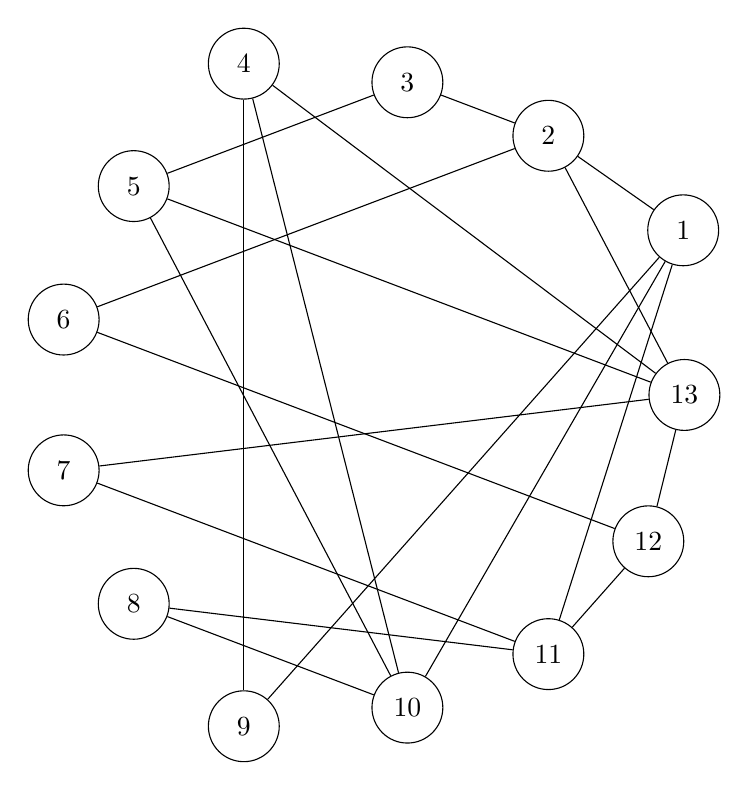
\begin{tikzpicture}

\node[circle,draw,minimum size=.9cm,color=black] (n1) at (27.69:4.5cm) { 1 } ;
\node[circle,draw,minimum size=.9cm,color=black] (n2) at (55.38:4cm) { 2 } ;
\node[circle,draw,minimum size=.9cm,color=black] (n3) at (83.08:4cm) { 3 } ;
\node[circle,draw,minimum size=.9cm,color=black] (n4) at (110.77:4.5cm) { 4 } ;
\node[circle,draw,minimum size=.9cm,color=black] (n5) at (138.46:4cm) { 5 } ;
\node[circle,draw,minimum size=.9cm,color=black] (n6) at (166.15:4cm) { 6 } ;
\node[circle,draw,minimum size=.9cm,color=black] (n7) at (193.85:4cm) { 7 } ;
\node[circle,draw,minimum size=.9cm,color=black] (n8) at (221.54:4cm) { 8 } ;
\node[circle,draw,minimum size=.9cm,color=black] (n9) at (249.23:4.5cm) { 9 } ;
\node[circle,draw,minimum size=.9cm,color=black] (n10) at (276.92:4cm) { 10 } ;
\node[circle,draw,minimum size=.9cm,color=black] (n11) at (304.62:4cm) { 11 } ;
\node[circle,draw,minimum size=.9cm,color=black] (n12) at (332.31:4cm) { 12 } ;
\node[circle,draw,minimum size=.9cm,color=black] (n13) at (360.00:4cm) { 13 } ;

\draw (n4) -- (n13) ;
\draw (n7) -- (n13) ;
\draw (n5) -- (n13) ;
\draw (n3) -- (n5) ;
\draw (n1) -- (n9) ;
\draw (n8) -- (n10) ;
\draw (n6) -- (n12) ;
\draw (n12) -- (n13) ;
\draw (n2) -- (n13) ;
\draw (n5) -- (n10) ;
\draw (n8) -- (n11) ;
\draw (n1) -- (n11) ;
\draw (n1) -- (n2) ;
\draw (n11) -- (n12) ;
\draw (n4) -- (n9) ;
\draw (n2) -- (n6) ;
\draw (n7) -- (n11) ;
\draw (n4) -- (n10) ;
\draw (n1) -- (n10) ;
\draw (n2) -- (n3) ;

\end{tikzpicture}
\end{center}

\subsection{Solution: Breadth-First Search Tree, with Bipartite Shading}

\[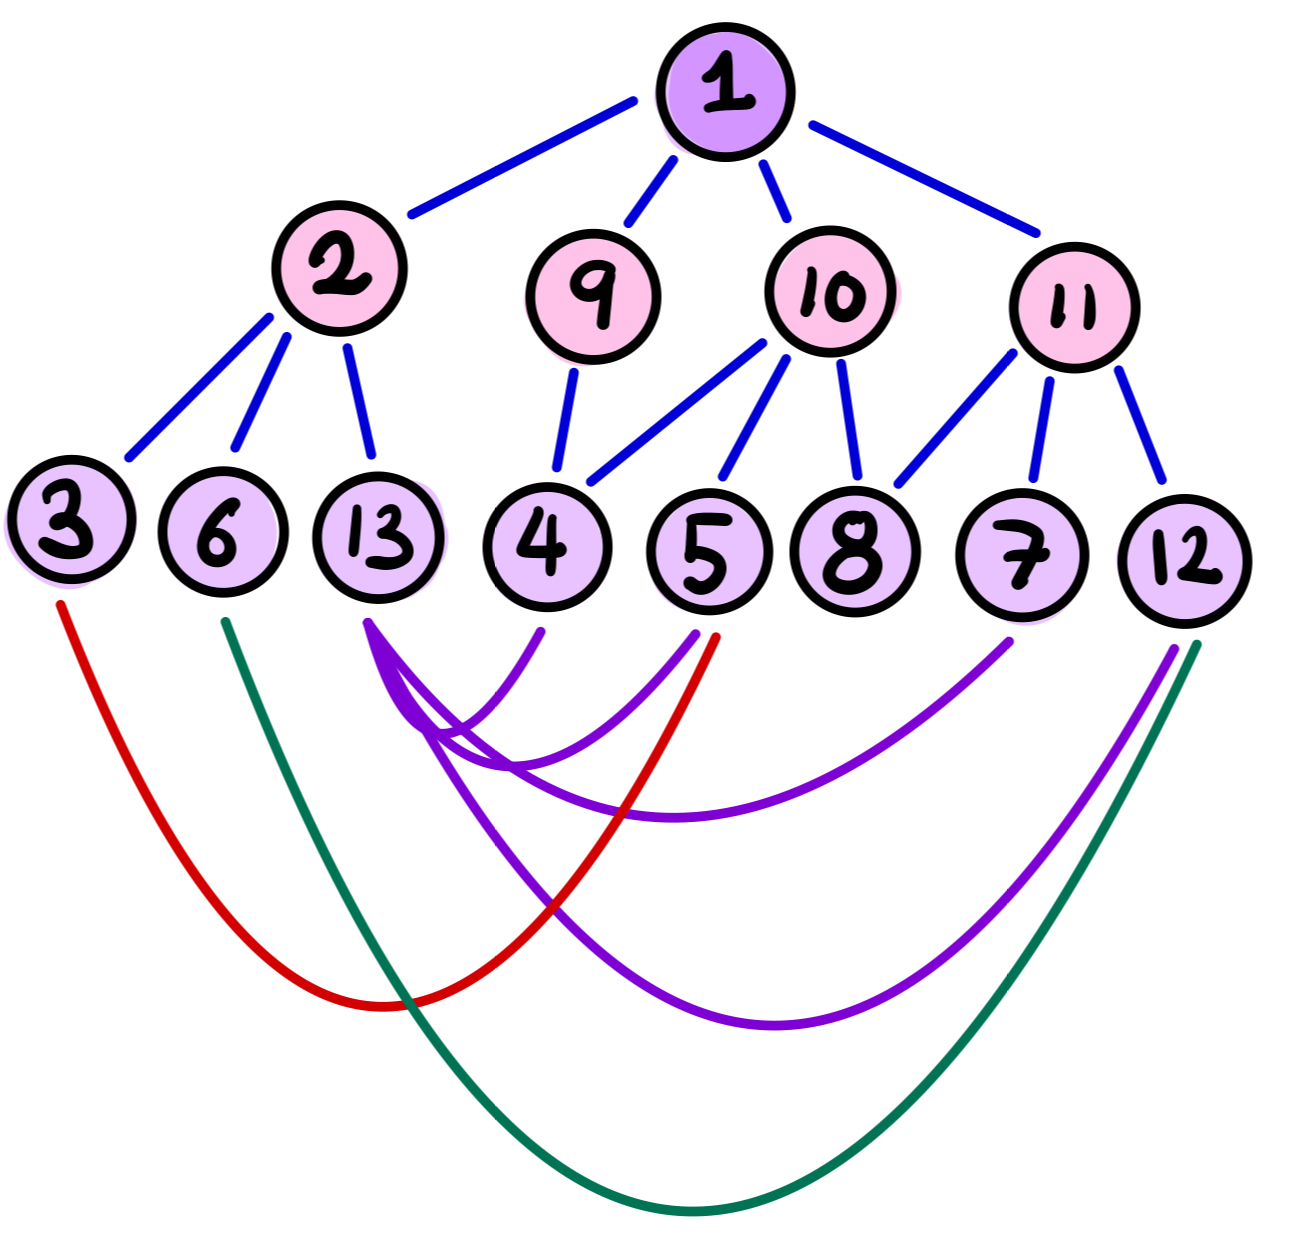
\includegraphics[width=9cm]{p1.jpg}\]

\[\text{Above: The BFS Tree created using root node }1 \text{ with attempted bipartite shading}\]

Because the tree above contains at least one odd cycle, for example, cycle containing nodes 1, 2, 3, 5, and 10, it is not bipartite.



\section{Topological Ordering (2 Points)}
Find a topological ordering of the Directed Acyclic Graph (DAG) shown below. Use numerical order with the smallest numbers first to break ties.

\begin{center}
  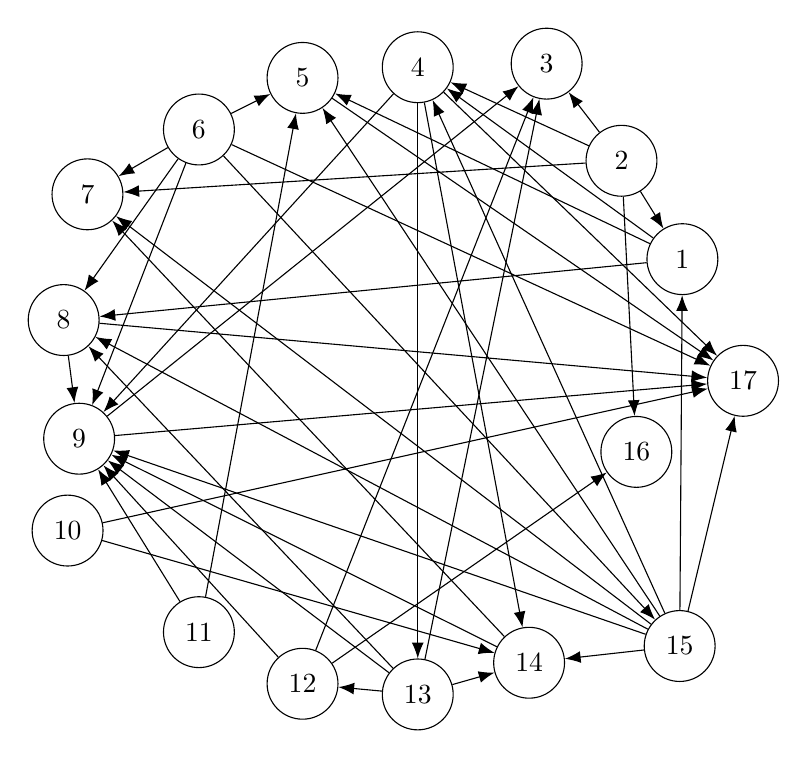
\begin{tikzpicture}
\node[circle,draw,minimum size=.9cm,color=black,yshift=.1cm] (n1) at (21.18:4cm) { 1 } ;
\node[circle,draw,minimum size=.9cm,color=black,yshift=.1cm] (n2) at (42.35:4cm) { 2 } ;
\node[circle,draw,minimum size=.9cm,color=black] (n3) at (63.53:4.5cm) { 3 } ;
\node[circle,draw,minimum size=.9cm,color=black] (n4) at (84.71:4cm) { 4 } ;
\node[circle,draw,minimum size=.9cm,color=black] (n5) at (105.88:4cm) { 5 } ;
\node[circle,draw,minimum size=.9cm,color=black] (n6) at (127.06:4cm) { 6 } ;
\node[circle,draw,minimum size=.9cm,color=black] (n7) at (148.24:4.5cm) { 7 } ;
\node[circle,draw,minimum size=.9cm,color=black] (n8) at (169.41:4.2cm) { 8 } ;
\node[circle,draw,minimum size=.9cm,color=black] (n9) at (190.59:4cm) { 9 } ;
\node[circle,draw,minimum size=.9cm,color=black] (n10) at (205:4.5cm) { 10 } ;
\node[circle,draw,minimum size=.9cm,color=black] (n11) at (232.94:4cm) { 11 } ;
\node[circle,draw,minimum size=.9cm,color=black] (n12) at (254.12:4cm) { 12 } ;
\node[circle,draw,minimum size=.9cm,color=black] (n13) at (275.29:4cm) { 13 } ;
\node[circle,draw,minimum size=.9cm,color=black] (n14) at (296.47:4cm) { 14 } ;
\node[circle,draw,minimum size=.9cm,color=black] (n15) at (317.65:5cm) { 15 } ;
\node[circle,draw,minimum size=.9cm,color=black,xshift=-.7cm,yshift=.2cm] (n16) at (344:4cm) { 16 } ;
\node[circle,draw,minimum size=.9cm,color=black] (n17) at (360.00:4.5cm) { 17 } ;

\draw[-{Latex[length=2mm]}] (n2) -- (n1) ;
\draw[-{Latex[length=2mm]}] (n13) -- (n8) ;
\draw[-{Latex[length=2mm]}] (n4) -- (n9) ;
\draw[-{Latex[length=2mm]}] (n15) -- (n4) ;
\draw[-{Latex[length=2mm]}] (n15) -- (n5) ;
\draw[-{Latex[length=2mm]}] (n6) -- (n5) ;
\draw[-{Latex[length=2mm]}] (n13) -- (n12) ;
\draw[-{Latex[length=2mm]}] (n12) -- (n16) ;
\draw[-{Latex[length=2mm]}] (n11) -- (n5) ;
\draw[-{Latex[length=2mm]}] (n2) -- (n7) ;
\draw[-{Latex[length=2mm]}] (n2) -- (n4) ;
\draw[-{Latex[length=2mm]}] (n10) -- (n14) ;
\draw[-{Latex[length=2mm]}] (n15) -- (n9) ;
\draw[-{Latex[length=2mm]}] (n1) -- (n4) ;
\draw[-{Latex[length=2mm]}] (n13) -- (n14) ;
\draw[-{Latex[length=2mm]}] (n6) -- (n9) ;
\draw[-{Latex[length=2mm]}] (n1) -- (n8) ;
\draw[-{Latex[length=2mm]}] (n8) -- (n17) ;
\draw[-{Latex[length=2mm]}] (n4) -- (n14) ;
\draw[-{Latex[length=2mm]}] (n14) -- (n7) ;
\draw[-{Latex[length=2mm]}] (n15) -- (n17) ;
\draw[-{Latex[length=2mm]}] (n12) -- (n3) ;
\draw[-{Latex[length=2mm]}] (n10) -- (n17) ;
\draw[-{Latex[length=2mm]}] (n15) -- (n8) ;
\draw[-{Latex[length=2mm]}] (n15) -- (n1) ;
\draw[-{Latex[length=2mm]}] (n8) -- (n9) ;
\draw[-{Latex[length=2mm]}] (n15) -- (n7) ;
\draw[-{Latex[length=2mm]}] (n2) -- (n3) ;
\draw[-{Latex[length=2mm]}] (n2) -- (n16) ;
\draw[-{Latex[length=2mm]}] (n15) -- (n14) ;
\draw[-{Latex[length=2mm]}] (n14) -- (n9) ;
\draw[-{Latex[length=2mm]}] (n9) -- (n17) ;
\draw[-{Latex[length=2mm]}] (n1) -- (n5) ;
\draw[-{Latex[length=2mm]}] (n13) -- (n3) ;
\draw[-{Latex[length=2mm]}] (n6) -- (n15) ;
\draw[-{Latex[length=2mm]}] (n6) -- (n17) ;
\draw[-{Latex[length=2mm]}] (n12) -- (n9) ;
\draw[-{Latex[length=2mm]}] (n11) -- (n9) ;
\draw[-{Latex[length=2mm]}] (n4) -- (n17) ;
\draw[-{Latex[length=2mm]}] (n13) -- (n9) ;
\draw[-{Latex[length=2mm]}] (n6) -- (n8) ;
\draw[-{Latex[length=2mm]}] (n9) -- (n3) ;
\draw[-{Latex[length=2mm]}] (n4) -- (n13) ;
\draw[-{Latex[length=2mm]}] (n6) -- (n7) ;
\draw[-{Latex[length=2mm]}] (n5) -- (n17) ;

\end{tikzpicture}
\end{center}

\subsection{Solution:}

The topological ordering is: 2, 6, 10, 11, 15, 1, 4, 5, 13, 8, 12, 14, 7, 9, 3, 16, 17





\section{Detect a Cycle (5 Points)}
Give an algorithm to detect whether a given undirected graph contains a cycle. If the graph contains a cycle, then your algorithm should output a cycle. (It should not output all the cycles in the graph, just one cycle.) The running time of your algorithm should be $O(m + n)$ for a graph with $n$ nodes and $m$ edges.

\subsection{Algorithm Solution}

Pick a vertex V as a root and perform a Depth-First Search Algorithm, maintaining a tree T. During the creation of T during the Depth-First Search Algorithm, at each point, starting from root V, when we encounter an edge to a vertex we have not yet encountered, the new vertex is added to the tree, along with the edge from the parent to the vertex. When we encounter an edge that leads to a vertex we have seen before, we know that there is a cycle. Once we know that there is a cycle, we can return the cycle by tracing the path in the DFS tree backwards until the cycle is complete and displaying it in the correct order, taking linear time. If the Depth-First Search Algorithm completes without finding a repeat edge, that means there is no cycle. Each DFS Algorithm takes linear time as well, since each edge and vertex is only visited once.



\section{All paths go through $r_{\text{ome}}$ (8 points)}

There's a natural intuition that two nodes that are far apart in a communication network—separated by many hops have a more tenuous connection than two nodes that are close together. There are a number of algorithmic results that are based to some extent on different ways of making this notion precise. Here's one that involves the susceptibility of paths to the deletion of nodes.

Suppose that an $n$-node undirected graph $G = (V, E)$ contains two nodes $s$ and $t$ such that the distance between $s$ and $t$ is strictly greater than $\frac{n}{2}$.  Either prove or disprove there exists a node $r$ which is not equal to $s$ or $t$, such that deleting $r$ from $G$ will destroy all paths between $s$ and $t$.

Your solution should include both:
\begin{itemize}
\item Draw a $n$-node graph (for $n \ge 4$) where the shortest path between $s$ and $t$ is strictly greater than $\frac{n}{2}$.  You should use this part of the problem to develop an intuitive understanding of the graph's properties.  You are not required to type this part of your solution, you can submit a photo of a hand-drawn graph.\footnote{If you are using LaTeX, you can follow the instructions here \url{https://www.overleaf.com/learn/latex/Inserting_Images} to embed an image in LaTeX.}

  To get you started, here is an example 3-node graph containing nodes $s$, $t$, and $r$ as described above.

  \begin{center}
    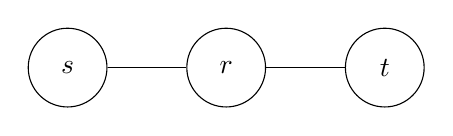
\begin{tikzpicture}[n/.style={draw,circle,minimum size=1cm}]
      \node[n] (s) {$s$} ;
      \node[n,right=of s] (r) {$r$} ;
      \node[n,right=of r] (t) {$t$} ;
      \draw[-] (s) -- (r) -- (t) ;
    \end{tikzpicture}
  \end{center}


\item Construct a proof or counterexample that exist a node $r$ for all graphs $G$ where distance between $s$ and $t$ is strictly greater than $\frac{n}{2}$ and that removing $r$ will destroy all paths between $s$ and $t$.

\end{itemize}

\subsection{Example Graph:}

\[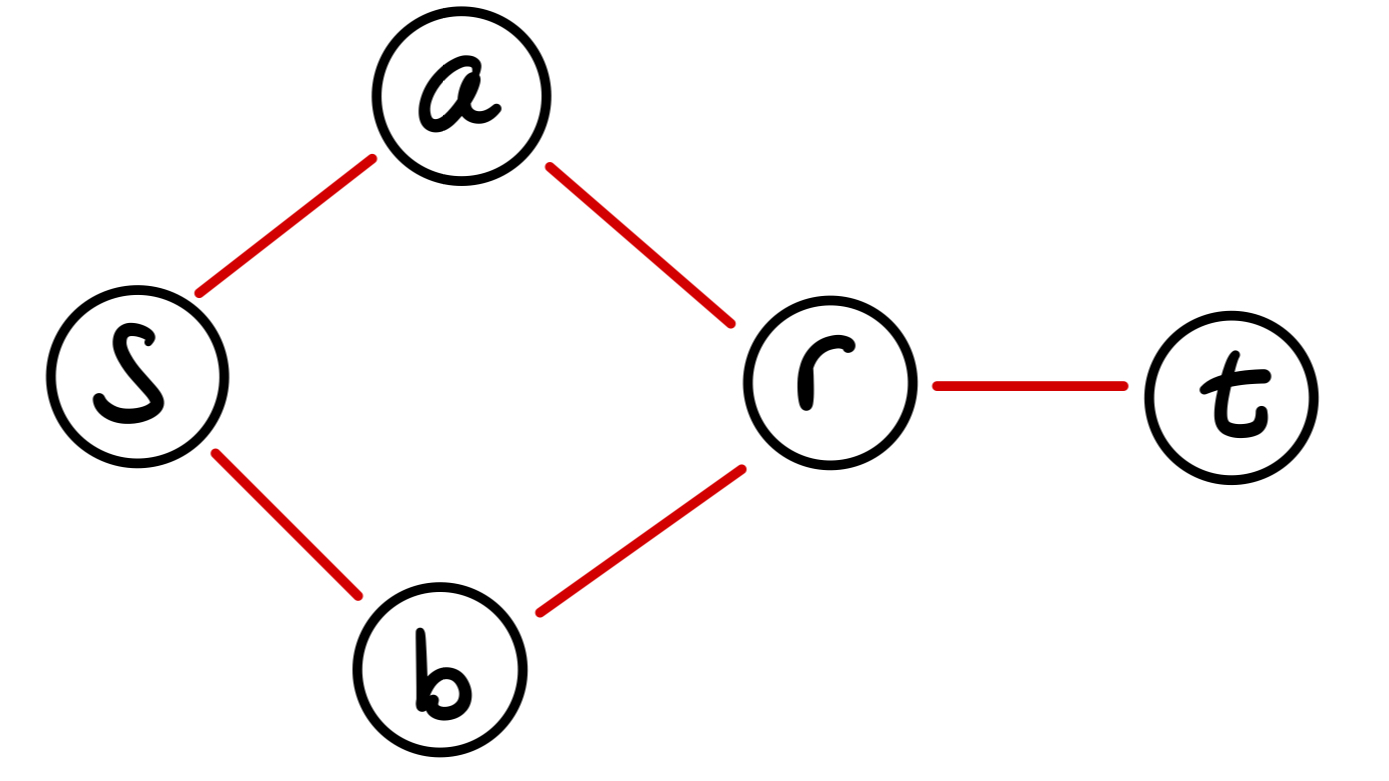
\includegraphics[width=9cm]{p4.jpeg}\]

Shown above is a graph with 5 nodes, where the shortest path between s and t are greater than 5/2 (3).

\subsection{Solution Proof:}

Let's use proof by contradiction. Assume there does not exist a node $r$ in the graph $G$ containing $n$ nodes such that removing $r$ destroys all paths between $s$ and $t$. From the claim above, the distance between $s$ and $t$ is greater than $\frac{n}{2}$, which means that there are at least $\frac{n}{2}$ nodes between nodes $s$ and $t$.

For the assumption to hold true that node r does not exist, there must be at least 2 nodes in every level so that more than one path exists to $t$ in every level. If we multiply $\frac{n}{2} * 2$, this gives us a total of $n$ nodes total in the layers between $s$ and $t$. Since we have not yet accounted for $s$ or $t$. This means that there are $n + 2$ nodes total in the entire graph.

Therefore, we must have a contradiction, since we stated that G contains $n$ nodes. Therefore, there can't be at least 2 nodes in every layer, which means that there exists at least one layer that only consists of one node which we can call node $r$. Deleting $r$ will delete all paths from $s$ to $t$ because there are no other nodes int eh alyer that $r$ resides in so all $s$ - $t$ paths are broken. Therefore, we have proven that such a node $r$ from the claim above exists.




\section{Some Short Paths in a Graph (8 points)}

A number of art museums around the country have been featuring work by an artist named Mark Lombardi (1951–2000), consisting of a set of intricately rendered graphs. Building on a great deal of research, these graphs encode the relationships among people involved in major political scandals over the past several decades: the nodes correspond to participants, and each edge indicates some type of relationship between a pair of participants. And so, if you peer closely enough at the drawings, you can trace out ominous-looking paths from a high-ranking U.S. government official, to a former business partner, to a bank in Switzerland, to a shadowy arms dealer.

Such pictures form striking examples of social networks, which, as we discussed in book chapter 3.1, have nodes representing people and organizations, and edges representing relationships of various kinds. And the short paths that abound in these networks have attracted considerable attention recently, as people ponder what they mean. In the case of Mark Lombardi's graphs, they hint at the short set of steps that can carry you from the reputable to the disreputable.


Of course, a single, spurious short path between nodes $v$ and $w$ in such a network may be more coincidental than anything else; a large number of short paths between $v$ and $w$ can be much more convincing.  So in addition to the problem of computing a single shortest $v$-$w$ path in a graph $G$, social networks researchers have looked at the problem of determining the number of shortest $v$-$w$ paths.


This turns out to be a problem that can be solved efficiently. Suppose we are given an undirected graph $G = (V, E)$, and we identify two nodes $v$ and $w$ in $G$. Give an algorithm that computes the number of shortest $v$-$w$ paths in $G$. (The algorithm should not list all the paths; just the number suffices.) The running time of your algorithm should be $O(m + n)$ for a graph with n nodes and m edges.  \\

Demonstrate your algorithm working on the graph given below.

\begin{center}
  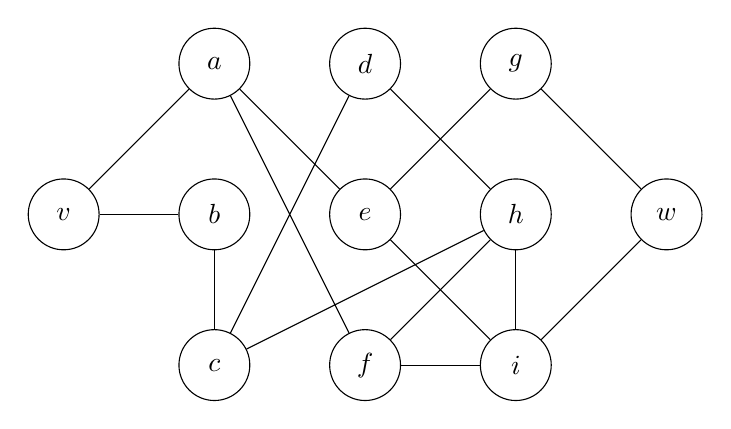
\begin{tikzpicture}[n/.style={draw,circle,minimum size=.9cm}]
    \node[n] (v) {$v$} ;
    \node[n,right=of v] (b) {$b$};
    \node[n,above=of b] (a) {$a$};
    \node[n,below=of b] (c) {$c$};

    \node[n,right=of b] (e) {$e$};
    \node[n,above=of e] (d) {$d$};
    \node[n,below=of e] (f) {$f$};

    \node[n,right=of e] (h) {$h$};
    \node[n,above=of h] (g) {$g$};
    \node[n,below=of h] (i) {$i$};

    \node[n,right=of h] (w) {$w$};

    \draw[-] (v) -- (a) -- (e) -- (i) -- (w) ;
    \draw[-] (v) -- (b) -- (c) ;
    \draw[-] (e) -- (g) -- (w) ;
    \draw[-] (a) -- (f) -- (h) -- (d) -- (c) -- (h) ;
    \draw[-] (f) -- (i) -- (h) ;
  \end{tikzpicture}
\end{center}

\subsection{Solution: Algorithm to Calculate the Number of Shortest Paths between Two Vertices}

\indent \indent Mark all nodes and edges in graph $G$ UNVISITED except starting node $v$;

\indent Introduce 2 arrays, shortestDistance[] which contains the length of the shortest path from the starting node to the current node, and shortestPaths[] which contains the number of shortest paths from the starting node to the current node. Set every shortestDistance[] to infinity, and set every shortestPaths[] to 0. Then, set shortestPaths[] of the root node as 1, and shortestDistance[] as 0.

\indent WHILE there exists an unvisited node $Z$ \{

\indent \indent FOR every neighbor node of the current node and every neighbor node after that \{

\indent \indent \indent IF the node is unvisited, mark as visited;

\indent \indent \indent IF (shortestDistance[neighbor node] $>$ shortestDistance[current node] + 1) \{

\indent \indent \indent \indent shortestDistance[neighbor node] = shortestDistance[current node] + 1;

\indent \indent \indent \indent shortestPaths[neighbor node] = shortestPaths[current node];

\indent \indent \indent \}

\indent \indent \indent IF (shortestDistance[neighbor node] = shortestDistance[current node] + 1) \{

\indent \indent \indent \indent shortestPaths[neighbor node] += shortestPaths[current node];

\indent \indent \indent \}

\indent \indent \}

\indent \}

\subsection{Solution: Algorithm Performed on Graph}

Suppose we want to find the number of shortest paths from vertex $v$ to $w$ in the above graph. The algorithm works as follows:

Consider source node $v$. shortestPaths[$v$] = 1, shortestDistance[$v$] = 0.

Go to node $a$. Mark visited. shortestDistance[$a$] = 1. shortestPaths[$a$] = 1.

Go to node $b$. Mark visited. shortestDistance[$b$] = 1. shortestPaths[$b$] = 1.

Go to node $e$. Mark visited. shortestDistance[$e$] = 2. shortestPaths[$e$] = 1.

Go to node $f$. Mark visited. shortestDistance[$f$] = 2. shortestPaths[$f$] = 1.

Go to node $c$. Mark visited. shortestDistance[$c$] = 2. shortestPaths[$c$] = 1.

Go to node $g$. Mark visited. shortestDistance[$g$] = 3. shortestPaths[$g$] = 1.

Go to node $i$. Mark visited. shortestDistance[$i$] = 3. shortestPaths[$i$] = 1.

Go to node $h$. Mark visited. shortestDistance[$h$] = 3. shortestPaths[$h$] = 1.

Go to node $d$. Mark visited. shortestDistance[$d$] = 3. shortestPaths[$d$] = 1.

Go to node $h$. shortestDistance[$h$] = 3. shortestPaths[$h$] = 2.

Go to node $i$. shortestDistance[$i$] = 3. shortestPaths[$i$] = 2.

Go to node $w$. shortestDistance[$w$] = 4. shortestPaths[$w$] = 1.

Go to node $w$. shortestDistance[$w$] = 4. shortestPaths[$w$] = 2.

Go to node $i$. shortestDistance[$i$] = 3. shortestPaths[$i$] = 2.

Go to node $w$. shortestDistance[$w$] = 4. shortestPaths[$w$] = 3.

Go to node $h$. shortestDistance[$h$] = 3. shortestPaths[$h$] = 2.

Go to node $i$. shortestDistance[$i$] = 3. shortestPaths[$i$] = 2.

Go to node $w$. shortestDistance[$w$] = 4. shortestPaths[$w$] = 3.

Return shortestPaths[$w$], which is 3. There are 3 shortest paths from $v$ - $w$.



\section{Wireless Network Connectivity (5 points)}

Some friends of yours work on wireless networks, and they're currently studying the properties of a network of $n$ mobile devices. As the devices move around (actually, as their human owners move around), they define a graph at any point in time as follows: there is a node representing each of the $n$ devices, and there is an edge between device $i$ and device $j$ if the physical locations of $i$ and $j$ are no more than 500 meters apart. (If so, we say that $i$ and $j$ are ``in range'' of each other.)

They'd like it to be the case that the network of devices is connected at all times, and so they've constrained the motion of the devices to satisfy the following property: at all times, each device $i$ is within 500 meters of at least $n/2$ of the other devices. (We'll assume $n$ is an even number.)  What they'd like to know is: Does this property by itself guarantee that the network will remain connected?


Here's a concrete way to formulate the question as a claim about
graphs.\\

\emph{Claim: Let $G$ be a graph on $n$ nodes, where $n$ is an even number. If every node
of $G$ has degree at least $n/2$, then $G$ is connected.}\\

Decide whether you think the claim is true or false, and give a proof of
either the claim or its negation.

\subsection{Solution: Proof by Contradiction}

Proof: We will consider a graph $G$ with all the mentioned properties in the problem above. Let's assume, for the sake of contradiction, that graph $G$ is not connected. In order for $G$ to be not connected, there has to be at least one node in $G$ that is isolated from the rest of $G$. \\

However, according to the claim above, every node has to have edges to at least $\frac{n}{2}$ other nodes. This means that these $(\frac{n}{2} + 1)$ nodes form a connected section of the graph that is disconnected from the other components. Let's call this section $S$. \\

If $S$ is a connected section of the graph and contains $(\frac{n}{2} + 1)$ nodes, the other connected section of the graph, which we will call $S'$, must contain $n - (\frac{n}{2} + 1) = \frac{n}{2} - 1$ nodes. \\

However, these $\frac{n}{2} - 1$ nodes cannot from a separate connected component $S'$ among themselves, since every node in $G$ must have edges to $\frac{n}{2}$ other nodes. Because of this, every node in $S'$ should have at least one edge to a node in $S$. Therefore, we have a contradiction. \\

Every node in $S'$ must be connected to at least one node in $S$. Therefore, A and B are connected, which contradicts our original assumption that G is disconnected. \\

Conclusion: If $G$ follows the given conditions, $G$ must be connected. \\


\end{document}
